% vim:autoindent:set textwidth=78:

\section{Der erste Einstieg}\label{label_getstarted}

% when the revision of a section has been finalized, 
% comment out the following line:
% \updatedisclaimer

Dieses Kapitel gibt eine kurze Einf�hrung in die Installation von QGIS,
verweist auf Alaska-Beispieldaten von der QGIS Webseite und zeigt anhand
eines einfachen Beispiels, wie einfach es ist, Raster- und Vektordaten in
QGIS zu visualisieren.   

\subsection{Installation}\label{label_installation}
\index{installation}

Die Installation von QGIS ist sehr einfach. Standard Installationspakete gibt
es f�r MS Windows und Mac OS X. F�r viele GNU/Linux Betriebssysteme stehen
Bin�rpakete (.rpm und .deb) oder entsprechende Software Repositories zur
Verf�gung, die man im Installationsmanager des jeweiligen Betriebsystems
eintragen kann. Aktuelle Informationen zu den Bin�rpaketen finden sich auf
der QGIS Webseite unter \url{http://qgis.osgeo.org/download/}.

Wenn Sie QGIS aus dem Quellcode kompilieren wollen, finden Sie die
entsprechende Dokumentation in Appendix \ref{sec:install_windows} f�r MS
Windows \win, Appendix \ref{sec:install_macosx} f�r Mac OSX \osx und
Appendix \ref{sec:install_linux} f�r GNU/Linux \nix. Die
Installationsanweisungen sind ausserdem im QGIS-Quellcode enthalten und �ber
die QGIS Webseiten unter \url{http://qgis.osgeo.org} verlinkt.

\subsection{Beispieldaten}\label{label_sampledata}
\index{data!sample} 

Die Dokumentation zeigt eine Reihe von Beispielen, die auf den Geodaten des
QGIS Beispieldatensatzes basieren. 

\win W�hrend der Installation unter Windows gibt es die Option, den QGIS
Beispieldatensatz mit herunterzuladen. Wenn die Option ausgew�hlt wurde,
werden die Daten nach \filename{Eigene Dateien} in einen Ordner \filename{GIS
Database} heruntergeladen. Mit dem Windows Explorer k�nnen Sie die Daten bei
Bedarf nachtr�glich in ein anderes Verzeichnis verschieben. Wenn Sie die
Option bei der Installation nicht ausgew�hlt haben, k�nnen Sie
\begin{itemize}
\item bereits auf Ihrem Rechner vorhandene GIS Daten verwenden;
\item den QGIS Beispieldatensatz nachtr�glich von der QGIS Webseite
\url{http://qgis.osgeo.org/download} herunterladen; oder
\item QGIS deinstallieren und wieder neu installieren und dabei die
entsprechende Option ausw�hlen.
\end{itemize}

\nix \osx F�r GNU/Linux und Mac OSX wird momentan noch kein fertiges
Installationspaket f�r den Beispieldatensatz als rpm, deb or dmg
bereitgestellt. Sie m�ssen daher die Datei \filename{qgis\_sample\_data} als
ZIP- oder TAR-Archiv von der URL \url{http://download.osgeo.org/qgis/data/}
herunterladen und auf Ihrem Rechner entpacken. 

Der QGIS Beispieldatensatz enth�lt Geodaten von Alaska und deckt s�mtliche
�bungen und Screenshots dieser Dokumentation ab, inklusive einer kleinen
GRASS GIS Datenbank. Das Koordinatensystem der Alaska Beispieldaten ist
Albers Equal Area mit der Ma�einheit 'feet'. Der EPSG-Code ist 2964.

\begin{verbatim}
PROJCS["Albers Equal Area",
    GEOGCS["NAD27",
        DATUM["North_American_Datum_1927",
            SPHEROID["Clarke 1866",6378206.4,294.978698213898,
                AUTHORITY["EPSG","7008"]],
            TOWGS84[-3,142,183,0,0,0,0],
            AUTHORITY["EPSG","6267"]],
        PRIMEM["Greenwich",0,
            AUTHORITY["EPSG","8901"]],
        UNIT["degree",0.0174532925199433,
            AUTHORITY["EPSG","9108"]],
        AUTHORITY["EPSG","4267"]],
    PROJECTION["Albers_Conic_Equal_Area"],
    PARAMETER["standard_parallel_1",55],
    PARAMETER["standard_parallel_2",65],
    PARAMETER["latitude_of_center",50],
    PARAMETER["longitude_of_center",-154],
    PARAMETER["false_easting",0],
    PARAMETER["false_northing",0],
    UNIT["us_survey_feet",0.3048006096012192]]
\end{verbatim}

Wenn Sie QGIS �berwiegend als grafische Benutzeroberfl�che f�r GRASS GIS
verwenden m�chten, finden Sie weitere Beispiel GRASS GIS Datenbanken (z.B.:
Spearfish oder South Dakota) auf der offiziellen GRASS Website unter
\url{http://grass.osgeo.org/download/data.php}. 

\subsection{Ein erstes �bungsbeispiel}\label{samplesession}

Nachdem Sie QGIS installiert und den Beispieldatensatz heruntergeladen und
entpackt haben, beginnen wir mit einem einfachen und kurzen Beispiel. Ziel
ist es, einen Raster- und einen Vektorlayer zu laden und wir verwenden dazu
den Rasterlayer \filename{qgis\_sample\_data/raster/landcover.img} und den
Vektorlayer \filename{qgis\_sample\_data/gml/lakes.gml} aus dem QGIS
Beispieldatensatz.

\minisec{QGIS starten}

\begin{itemize}
\item \nix{Starten Sie QGIS, indem Sie \usertext{qgis} in ein
Kommandozeilenfenster tippen und denn Return dr�cken.}
\item \win{Starten Sie QGIS �ber das Start Men�, das QGIS Desktop Icon oder
durch doppelklicken auf eine evtl. bereits vorhandene QGIS Projektdatei.}
\item \osx{Doppelklicken Sie auf das QGIS Icon in Ihrem Programmordner.}
\end{itemize} 

\minisec{Laden eines Raster- und Vektorlayers aus dem Beispieldatensatz}

\begin{enumerate}
\item Dr�cken Sie auf den \toolbtntwo{mActionAddRasterLayer}{Rasterlayer
hinzuf�gen} Knopf.
\item Browsen Sie zum Ordner \filename{qgis\_sample\_data/raster/}, w�hlen
Sie die ERDAS Img Datei \filename{landcover.img} und klicken dann auf
\button{�ffnen}.
\item Nun dr�cken Sie auf den \toolbtntwo{mActionAddOgrLayer}{Vektorlayer
hinzuf�gen} Knopf.
\item Browsen Sie zum Ordner \filename{qgis\_sample\_data/gml/}, w�hlen Sie
die GML Datei \filename{lakes.gml} aus und klicken auf \button{�ffnen}.
\item Zoomen Sie in einen Bereich in dem sich ein paar Seen befinden.
\item Doppelklicken Sie auf das Wort \filename{lakes} in der Legende, um die
den Dialog zur Einstellung der \dialog{Layereigenschaften} zu �ffnen.
\item Klicken Sie auf den \tab{Darstellung} Reiter und w�hlen Sie die Farbe
Blau als F�llfarbe.
\item Klicken Sie auf den \tab{Beschriftungen} Reiter und aktivieren Sie die
\checkbox{Zeige Beschriftungen an} Checkbox.
\item Dr�cken Sie nun auf \button{Anwenden}.
\end{enumerate} 

\begin{figure}[ht]
   \begin{center}
   \caption{Eine einfache QGIS Beispiel�bung \nixcaption}\label{fig:simple_session}\smallskip
   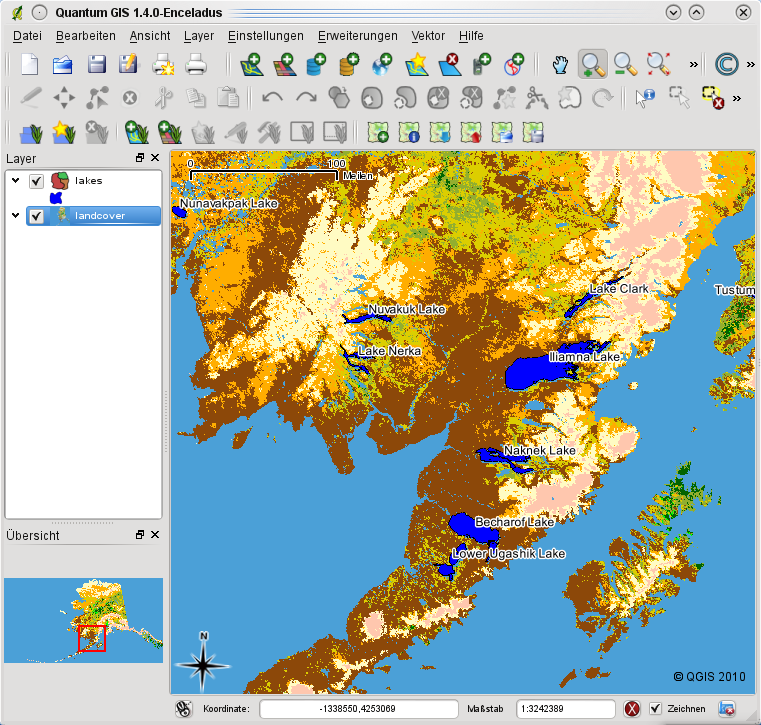
\includegraphics[clip=true, width=14cm]{simple_session}
\end{center}  
\end{figure}

Sie sehen, wie einfach es ist, Raster- und Vektorlayer in QGIS zu
visualisieren. Gehen Sie nun weiter zu den folgenden Kapiteln, um mehr �ber
die vorhandenen Funktionalit�ten, Einstellungsm�glichkeiten und ihre
Benutzung zu erfahren. 
